% Chapter 1

\chapter{Introduction} % Write in your own chapter title
\label{Chapter1}
%\lhead{Chapter 1. \emph{Introduction}} % Write in your own chapter title to set the page header
Imagine Anna who studies Russian language and history. She reads a book `Rossija, krov'ju umytaja' by Art\"{e}m Ves\"{e}lyj  and comes across the sentence \ref{ex:dovybirali}.

\exg.\label{ex:dovybirali}Okolo pravlenija, po predlo\v{z}eniju Banty\v{s}a, dovybirali \v{c}lena rady.\\
near administration.\glb{sg.gen} along proposal.\glb{sg.dat} Bantysh.\glb{gen} do.vy.take.imp.\glb{pst.pl} member rada.\glb{gen}\\
\vspace{0.3em}
`Near the administration building, following the proposal by Bantysh, a rada member was being elected.'

Anna looks in her Russian dictionary and does not find the verb \textit{dovybirat'} `to finish electing/to elect in addition' there.  What she can find is the verb \textit{vybrat'} `to select'  that has one prefix and one suffix less and is perfective. Anna knows that the semantic contribution of the prefix \textit{do-} is similar to `finish', but what she does not know is the aspect of the verb she encountered in \ref{ex:dovybirali}. 

Anna remembers from her Russian classes that one can form perfective verbs by prefixation and imperfective verbs by attaching the imperfective suffix. This case, however, is different, as the verb contains two prefixes and the imperfective suffix. There are, thus, two possibilities for the order of affix attachment: first two prefixes and then the suffix, or one prefix, the suffix, and the other prefix. These two possibilities are, however, associated with different aspect of the derived verb. The questions what does this verb mean and what is its aspect remain unanswered. If `dovybirali' is perfective, it must refer to a completed event of electing. If it id imperfective, it could refer to the process of finishing the elections (which it, in fact, does), or to a repeated event of electing. 

Surprisingly, not only Russian grammar and dictionaries, but also linguistic literature does not provide a full answer to these questions. For example, the proposals by \citet{Svenonius:04b} and \citet{Tatevosov:07} predict different internal structure and aspect of the verb \textit{dovybirat'}: according to \citet{Svenonius:04b}, the prefix \textit{do-} is attached last and the verb is perfective, and according to \citet{Tatevosov:07}, both steps of prefixation precede the suffixation, so the verb is imperfective.

As the predictions of two proposals do not coincide, it seems an easy task to find out which one is wrong: one has to apply tests that are used to determine the aspect of the verb and check which prediction is correct. These tests are based on the ability of imperfective verbs to receive a progressive interpretation in non-past tense, a habitual interpretation in past tense, and to be combined with the auxiliary verb \textit{budet} `will'. All these properties, however, allow to identify perfective verbs only in terms of the absence of imperfective characteristics. The prob;em is the existence of biaspectual verbs: verbs that, depending on the context, can be used either as perfective or as imperfective. This means that standard tests in principle fail to identify biaspectual verbs, because they result being in one class with imperfective verbs.

In Chapter~\ref{Chapter2} I develop a possible positive test for perfectivity and show that in case of verbs like \textit{dovybirat'} both \citet{Svenonius:04b} and \citet{Tatevosov:07} are to some extent right and wrong at the same time: both derivations (and thus aspects) are possible, but either theory fails to predict their coexistence. Learning from this, in Chapter~\ref{Chapter2}, I not only present new data that is problematic for the existent analyses, but also develop a systematic approach that allows to collect and analyse data independently from the theoretical view on the structure of complex verbs in Russian. I then show that, if this approach is adopted, it provides evidence for structural ambiguity in some cases where no aspectual ambiguity is present, so the class of verbs that require reanalysis with respect to the established syntactic approaches to prefixation is broadened.\footnote{Parts of Chapter~\ref{Chapter2} has been published as \citealt{ZinovaFilip:13} and \citealt{ZinovaOsswald:paper}.}

Another puzzling issue arises in situations when the predictions of different analyses (e.g., \citealt{Svenonius:04b} and \citealt{Tatevosov:07}) agree but depend on the interpretation of the prefix. This happens, for example, if the verb contains the imperfective suffix and two prefixes, whereby the leftmost prefix is \textit{pere-}, as in the verb \textit{perevybirat'} `to be reelecting/to elect all of'. How can one find out which interpretations are available for the given verb? 

Traditional descriptive approaches, adopted in grammars and dictionaries such as \citet{Shvedova:82}, provide information about the range of interpretations a given prefix may receive, but do not indicate in which situation which interpretation applies, unless the derived verb is itself present in the dictionary. The most extensive and detailed analysis of prefix semantics in formal terms is proposed in the recent book by \citet{Kagan:book}. The goal of the study by \citet{Kagan:book} is to unify prefix representations on two levels: first, all prefixes receive scalar semantic analysis and second, each prefix is assigned a common core meaning from which different interpretations can be derived. 

\citet{Kagan:book}, however, does not aim to distinguish between the situations where different submeanings arise nor to explain prefix combinatorics and interaction with the imperfective suffix. This means that despite the unified representation one still cannot derive the exact meaning of the prefixed verb in a given sentence, as this would require more details about how the context influences the interpretation of the verb.

In this work, I provide representations that allow to derive both the aspect and the semantics of a given verb. I also aim to predict which combinations of affixes are possible and formulate the rules that govern complex verb formation in Russian. According to \citet{Shvedova:82}, there are 23 productive prefixes in Russian. They can stack and at some point of the derivation process the imperfective suffix can be attached. So in principle for each verbal stem there can be more than 20 thousand derived verbs, not taking into account polysemy of individual prefixes. However, from the point of view of a native speaker, the number of possible derivations seems much more restricted. The primary mean of explaining this restriction in the recent proposals is the division of all prefixes into \textit{lexical} and \textit{superlexical}. It originates from the proposal of \citet{Isachenko:60} and is advocated in such contemporary works on Russian prefixation as \citet{Ramchand:04}, \citet{Svenonius:04b}, \citet{Romanova:06}, and \citet{Tatevosov:07, Tatevosov:09}.

The main idea of the division is to assign all verbal prefixes to either lexical or superlexical class. Prefixes that belong to different classes are then associated with distinct structural positions. This allows to significantly limit the number of possible derived verbs. Surprisingly, different authors that consider that dividing prefixes into two classes is crucial for understanding Russian prefixation system, do not agree on how to perform this division, which has been noted already by \citet{Tatevosov:09}. It turns out that the assignment itself is controversial because the criteria that are used to identify which class a given prefix belongs to, are vague. In Chapter~\ref{Chapter4}, I discuss all of the properties that are typically assigned to verbs of either class and show that no pair of them is true of the same set of prefixes or prefix usages. Based on this, I argue that, despite the differences between the properties of certain prefixes, the view of a strict distinction is problematic and needs to be revised, probably in favour of a continuum between two extremes instead of a discrete classification. 

An implicit movement away from a bipartite distinction is, in fact, already present in papers that advocate the lexical/superlexical split: \citet{Svenonius:04b} allows different structural positions for various prefixes of the superlexical class, \citet{Tatevosov:07} argues for an additional class of intermediate prefixes, and \citet{Tatevosov:09} introduces a three-way classification among the superlexical prefixes. However, explicit rejection of the bipartite distinction leads to a radical change as it forces to abandon the hypothesis of distinct structural positions for different prefixes. This hypothesis, in turn, serves as a main limiting force in the syntactic accounts of verbal prefixation in Russian: it allows to provide a structure of a given complex verb and predict which affix combinations are impossible.

Instead of the criticized syntactic explanation of prefix combinatorics, I propose a formal semantic account that allows to make predictions and block derivations when semantic conflicts occur. In Chapter~\ref{Chapter5}, I prepare the ground for this formalization: I discuss relevant properties of some of the usages of prefixes \textit{\mbox{za-}}, \textit{na-}, \textit{po-}, \textit{pere-}, and \textit{do-}. The analysis I develop is based on the idea of scalar approach to verbal prefixation, proposed by \citet{Filip:08} and further elaborated by \citet{Kagan:12, Kagan:book}. In Chapter~\ref{Chapter5}, though, I mostly discuss data and provide generalizations based on it in order to do the formal modelling in Chapter~\ref{Chapter7}.

Working out the semantic contribution of prefixes makes it necessary to also account for pragmatic meaning components. The literature is inconclusive in this respect: \citep{Paducheva:96, Romanova:06} claim that all perfective verbs carry presuppositions, while \citet{Kagan:book} attributes this property only to the prefixes \textit{do-} and \textit{pere-}. In Chapter~\ref{Chapter6}, I discuss these hypotheses. I apply standard tests for presuppositions and show that perfective verbs in general are clearly not associated with a presupposition, as has been already noticed by \citet{Gronn:04}.\footnote{This part has been done together with Hana Filip and published as \citealt{ZinovaFilip:14}.}

Test results, however, do not provide a clear answer with respect to whether the prefixes \textit{do-} and \textit{pere-} carry presuppositions. To find out more, I collected data from native speakers of Russian using a special questionnaire. This questionnaire is based on the results of recent experimental work by \citet{Chemla:09}. After doing a statistical analysis of the results, I arrive at the conclusion that the idea of a presuppositional component carried by the prefixes has to be discarded. I then propose to model the observed inferences as entailments in positive contexts and scalar implicatures in negative contexts.\footnote{This part has been done together with Hana Filip and published as \citealt{ZinovaFilip:SALT}.}

In the same chapter, I discuss another pragmatic issue: competition of prefixed verbs derived from the same base. I show how by using underspecified semantics and basic pragmatic principles one can obtain distinct interpretations of the same prefix depending on the derivational base. Such interpretation variability is traditionally described as polysemy and the problem of finding which submeaning applies in the particular case has been not accounted for earlier. This part, however, remains at the level of a preliminary proposal and I hope to return to implementing it in the future work.

After the data analysis conducted in Chapter~\ref{Chapter5} and Chapter~\ref{Chapter6}, I propose formal semantic representations of the five Russian verbal prefixes in Chapter~\ref{Chapter7}. I show how they combine with the representations of the derivational bases and how the direct object contributes to the interpretation of the verbal phrase. I use a combination of frame semantics and Lexicalized Tree Adjoining Grammars as defined in \citealt{KallmeyerOsswald:13}. The choice of this formal framework is motivated by its flexibility in combination with the potential to express semantic restrictions. Another important factor of the framework selection is the possibility to provide an implementation of the analysis. 

The idea that drives the frame semantics approach \citep{Loebner:2014} is that frames in the sense of \citet{Barsalou:92} constitute the universal format of representaion of concepts. They are recursive attribute-value structures with functional attributes that can also be represented as directed graphs. Let me show the two graphs that emerge from my analysis for the verb \textit{dovybirat'} that Anna could not find in the dictionary.

\begin{figure}
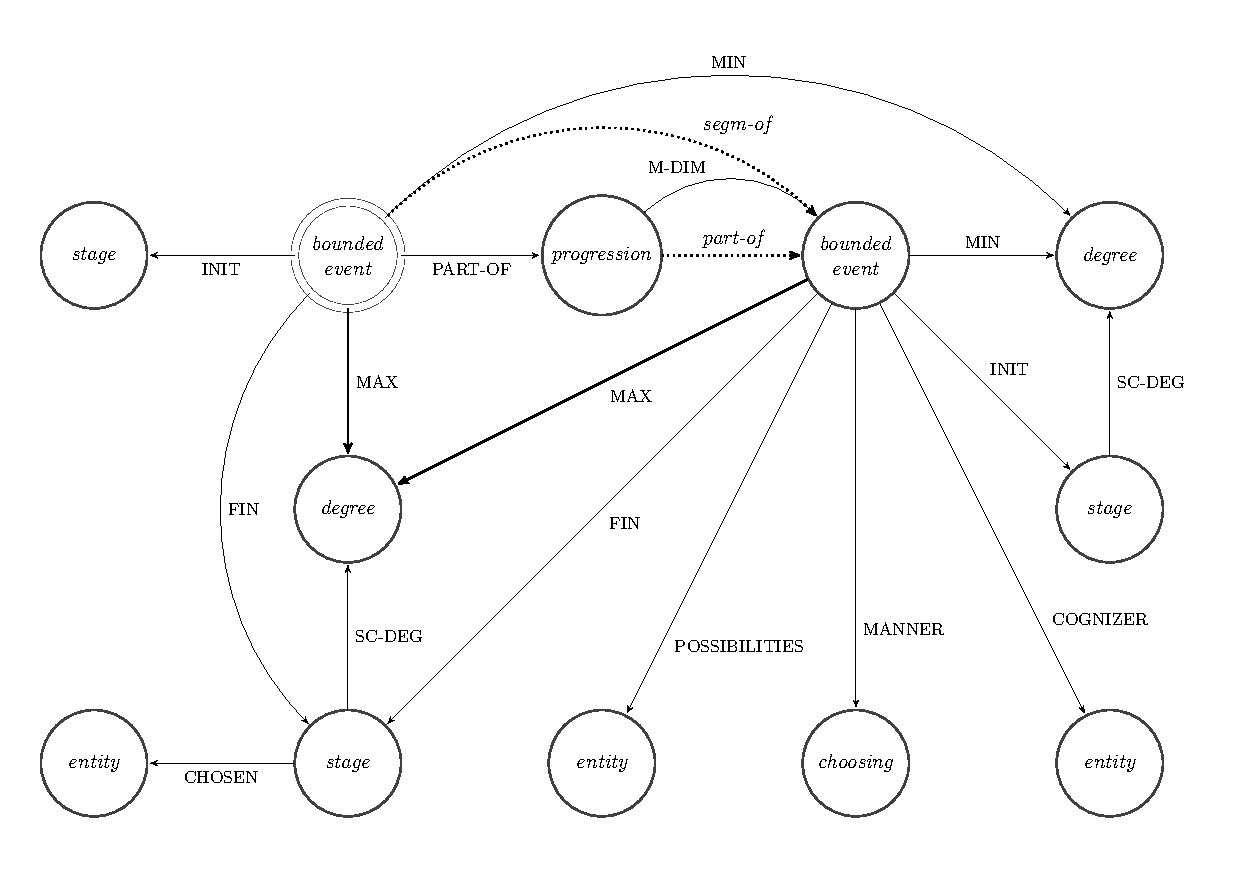
\includegraphics[width=\textwidth]{dovybiratpf.pdf}
\caption{Graph representation of the verb \textit{dovybirat'}$^{\PF}$ `to finish electing'}
\label{graph:pf}
\end{figure}

The first graph, shown on \figref{graph:pf}, represents the semantics of the verb \textit{dovybirat'}$^{\PF}$ `to finish electing' derived with first suffixing the verb \textit{vybrat'}$^{\PF}$ `to elect' and then prefixing it with \textit{do-}. The central node of the frame is of type \textit{bounded event} and is marked with a double circle. This event is a segment of the bounded event that is denoted by the verb \textit{vybrat'}$^{\PF}$ `to elect'. This is shown by a relation between the two nodes: a thicker arrow in the top part of the figure. These two event share the final stage (\FIN attribute) but have different initial stages (\INIT attribute). The final stage is at the same time the maximum of the event and the initial point of the derived event does not have to be the minimum of the event. This is interpreted as `to finish electing'. The frame also contains information related to the arguments and manner of the verb \textit{vybrat'}$^{\PF}$ `to elect', that I have taken from the FrameNet project\footnote{\url{https://framenet.icsi.berkeley.edu/fndrupal/}}: manner \textit{choosing}, a set of possibilities, a cognizer, and a chosen that I represent as an attribute of the final stage of the event.

\begin{figure}
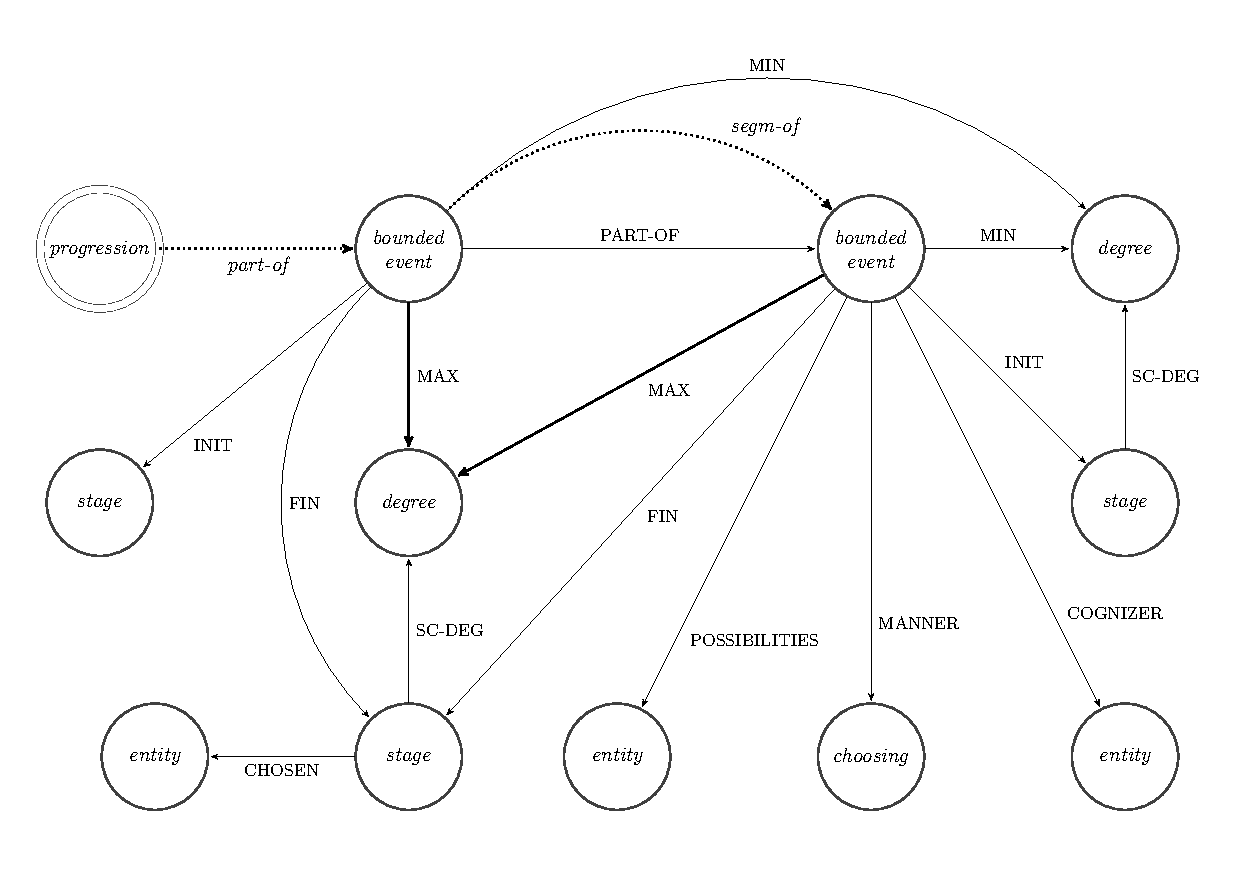
\includegraphics[width=\textwidth]{dovybiratipf.pdf}
\caption{Graph representation of the verb \textit{dovybirat'}$^{\IPF}$ `to be finishing electing'\label{graph:ipf}}
\end{figure}

The second frame, shown on \figref{graph:ipf}, shares a lot with the first one. However, the crucial difference can be immediately seen: the central node (marked with the double border of the circle) is now of type \textit{progression,} which provides an indication that the verb is imperfective. This is the case when the imperfective suffix is attached on the last step of the derivation. The derived verb, thus, denotes a partial event of electing that is, in turn, a segment of the whole electing event that contains its final stage. The attributes of the core electing event remain the same. 

The frame semantic analysis of Russian prefixation system that I develop in Chapter~\ref{Chapter7} illustrates the power and flexibility of the formalism: with basic and easily readable semantics I manage not only to provide the exact interpretation of a given prefixed verb in context, but also block unwanted derivations of complex verbs as well as prevent combinations of verbs with inappropriate direct objects and measure phrases.

I then implement the proposal using XMG 2 \citep{Petitjean:16}. In Chapter~\ref{Chapter8}, I show parts of the implementation and discuss technical details. Due to the current restrictions with respect to the tools available for parsing, I only implement a small fragment that consists of six prefix usages, one verbal base, the imperfective suffix, and one noun that can serve as a direct object, supplying two different scales. The output of the compiler consists of verb models that include various affixes. Each model is accompanied by a tree that shows its internal structure, a set of syntactic properties (including aspect), and a frame that represents the  semantics of the verbal phrase. This allows to check the predictions of the account I propose without the risk of overlooking an unwanted derivation or of making a mistake during the derivation of the representation of a complex verb. This is extremely important if one wants to explore verbs that contain three and more derivational affixes.

In order to see how well my analysis does with respect to predicting the (non-)existence of certain affix combinations, I compare the output of my analysis against the proposal by \citet{Tatevosov:09}. For this, I implement the syntactic restrictions for prefix attachment for the same grammar fragment. I then analyse all the models produced by the two implementations and calculate precision and recall. The comparison shows that both approaches rather accurately describe situations with one or two affixes, but both precision and recall of the model built following the proposal of \citet{Tatevosov:09} get low values due to the incorrect predictions of the existence of more complex verbs. As for the implementation of the approach I propose, it continues to deliver accurate predictions beyond two affix situations. In addition, the pragmatic reasoning I propose fine-tunes the system and allows to explain the non-existence of extra models produced by the implementation. From this it follows that with a three component analysis of Russian prefixation that I advocate in this thesis one can achieve full precision and recall in predicting the existence of complex verbs that are not lised in the dictionaries.

In sum, in this thesis I develop a complex system that allows to explain Russian prefixation and predict existence, aspectual properties, and semantics of complex verbs. The crucial idea of the analysis is the interaction between syntax, semantics, and pragmatics. While all the components are kept simple, their combination allows to explain subtle distinctions and cases that seem exceptional when all the work is assigned to one linguistic module. An important property of the analysis is the possibility to implement it, which is partially performed in this work.
